\chapter{Trabalhos Relacionados}
\label{cap:trabalhos-relacionados}
Este capítulo apresenta trabalhos que possuem relação com o tema proposto, resultantes do processo da Revisão Sistemática da Literatura. Neste capítulo o objetivo é apresentar o resumo dos 4 artigos selecionados e esclarecer qual o objetivo das pesquisas, os métodos utilizados e seus resultados.

\section{Facial skin colour classification using machine learning and hyperspectral imaging data} 

Segundo o estudo \cite{Facial_skin_colour_classification_using_machine_learning_and_hyperspectral_imaging_data}, a indústria da beleza enfrenta a falta de métodos precisos para classificar automaticamente a cor da pele, pois utiliza rótulos de granularidade alta, como a escala Pantone, a qual é utilizada na \textit{Skin Tone Guide} e abrange até 110 tipos de cor de pele facial. Neste contexto, o estudo examinou tecnologias projetadas para coletar dados de cores de pele, bem como métodos para classificar com precisão os tipos de cores de pele usando a escala Pantone como referência.
 
% Segundo o estudo \cite{Facial_skin_colour_classification_using_machine_learning_and_hyperspectral_imaging_data}, a indústria da beleza carece de métodos precisos para classificar automaticamente a cor da pele porque utiliza de rótulos de alta granularidade, como a escala Pantone utilizado na \textit{Skin Tone Guide} que detém até 110 tipos de cor de pele facial. Com isso, nesse estudo foi examinado tecnologias projetadas para coletar dados de cores de pele faciais e métodos para classificar com precisão os tipos de cores de pele faciais usando a escala Pantone como base.

A classificação automática da cor da pele do rosto foi realizada com base em imagens hiperespectrais e aprendizado de máquina.  A imagem hiperespectral, conhecida como imagem espectral ou química, é uma tecnologia de medição não invasiva usada para coleta de dados que já é utilizada para medir a saúde da pele. E, para auxiliar nisso, foi avaliado seis métodos de aprendizado de máquina aplicados a esses dados e comparados e descobriu-se que cada um tinha uma vantagem na categorização de um subconjunto de tipos de cores, além disso, foi abordado a classificação para a cromaticidade e brilho para alcançar a precisão mínima de 90\% de precisão.

A metodologia utilizada é referenciada como aprendizado de máquina \textit{offline} supervisionado, já que o tipo de cor correto é conhecido e baseado no Guia da Pantone, e os dados foram coletados antes do início do aprendizado. Contudo, o experimento teve desafios, principalmente ao  coletar \textit{big data} sobre a cor da pele do rosto por meio de imagens hiperespectrais para a classificação da cor da pele facial.  Primeiro desafio se referiu à coleta de dados multidimensionais nos diferentes tipos de cores de pele e à alta granularidade dos tipos de tom da pele. O segundo, ao classificar o tipo de cor com precisão, considerando que imagens espectrais são influenciadas por fatores ambientais. E, terceiro, ao escolher o melhor método de classificação projetados para classificar os tipos de cores faciais com base nos dados de imagens hiperespectrais de modo que alcancem precisão mínima esperada.

O experimento baseou-se na geração de imagens hiperespectrais em laboratório utilizando um gerador da marca Photon para registrar imagens de 108 tipos de cores do Guia Pantone de Tons de Pele, onde cada cor era representado por um cartão. A partir disso, os cartões eram iluminados com altura, distância, temperatura e umidade padrões, assim a luz incidida no cartão era refletida e capturada pelo equipamento. Cada cartão foi medido 20 vezes para minimizar a perda de dados. Apesar das medições repetidas, foi necessário analise e classificação  dos dados brutos para identificar possíveis anomalias nas medições, considerando a média das intensidades luminosas e as distâncias euclidianas entre a média de cada medição. Tendo como resultado das 2160 medições apenas 1725 medições válidas. Assim, para resolver a classificação dos tipos de cor foi explorado métodos de aprendizagem automática.

No estudo, foram utilizados oito classificadores com seis métodos de classificação diferentes em que foram comparados as suas taxas de precisão, sendo eles regressão logística, KNN, SVM com kernel linear, SVM com kernel radical, SVM com kernel polinomial, árvore de decisão, reforço adaptativo e floresta aleatória. Como pode ser visto na Figura \ref{fig:x classificacao} o método de floresta aleatória teve a precisão mais elevada de 88\%, seguida da SVM com função de kernel radical, reforço adaptativo e KNN acima de 50\%. Contudo, ao se comparar a diferença de precisão na classificação por tipos de cor, o método de regressão logística possuía a menor precisão para todos os tipos de cor entre os classificadores. E, os outros classificadores, exceto a regressão logística, obtiveram uma vantagem de precisão em diferentes tons de pele. Isso resultou na necessidade de integrar os métodos para melhorar a desempenho da precisão dos métodos escolhidos para a classificação de tipo de cor de pele facial.

\begin{figure}[h]
\centering
\caption{Precisão de classificação entre os oito classificadores}
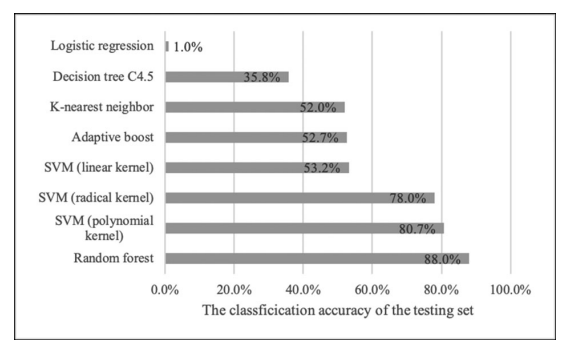
\includegraphics{Template_Latex_TCC-UNIFTEC/_lib/imagens/resultados_facial_skin.png}

\label{fig:x classificacao}
\centering{\Fonte{\cite{Facial_skin_colour_classification_using_machine_learning_and_hyperspectral_imaging_data}}}
\end{figure}

Para explorar os pontos fortes dos classificadores, foi proposto um classificador integrado de dois estágios que empilha seus resultados para produzir uma nova previsão e validação cruzada por 10 vezes. Na primeira etapa, foi utilizado sete classificadores usando um conjunto de treinamento e, em seguida, aplicado a outro conjunto de treinamento. As saídas dos classificadores formam uma nova entrada independente de sete dimensões atributos.  Na segunda etapa, foi utilizado o conjunto de treinamento para construir uma floresta aleatória empilhada classificador. A partir disso, a segunda abordagem proposta alcançou 89,4\% de precisão no conjunto de teste. Esta foi uma ligeira melhoria em relação à precisão de 88,0\% do classificador básico de floresta aleatória, mas ainda ficou aquém da exigência prática de 90\% de precisão.

Ao analisar as características dos dados coletados descobriu-se que a cromaticidade e o brilho da pele podem ser classificados separadamente, e fornecem informações relevantes. Por isso, para melhorar mais a precisão  dos dados, eles foram classificados conforme o tipo de cor. Cada tipo de cor de cartão foi dividido em subtipos de cromaticidade e brilho. A cromaticidade mede a qualidade da cor, e o brilho mede a intensidade da luz e segundo o Guia Pantone de Tom de pele há 10 classes de cromaticidade e 15 classes de brilho.

A classificação de subtipos por cromaticidade permitiram refinar os classificadores melhorando a precisão, já que houve diferenças discrepantes entre elas, sendo que algumas que exibiram menor intensidade e outras maiores intensidade em todos os espectros. Isso resultou no aumento da precisão no método floresta aleatória para 95,9\% o que pode ser visto na Tabela \ref{table:Tabela_comparativa_entre_os_métodos_e_precisões}.

Já a classificação de subtipos por brilho considerou 15 espectros de brilho. Os dados mostraram que o nível mais altos sofreram mais distinção que os outros, contudo eles acabaram criando cluster entre os níveis. Contudo, a classificação do subtipo de brilho foi significativamente menos precisa. Assim, os subtipos de brilho foram mais difíceis de distinguir um do outros em comparação com a cromaticidade.


\begin{table}[]
\centering
\caption{Tabela comparativa entre os métodos e precisões}
\label{table:Tabela_comparativa_entre_os_métodos_e_precisões}\textbf{}
\resizebox{\columnwidth}{!}{%
\begin{tabular}{lllll}
\hline
Algoritmo classificador & Precisão & Precisão por nível de cromaticidade & Precisão por nível de brilho &  \\ \hline
Regressão Logística     & 1.0\%    & -                                   & -                            &  \\
Árvore de decisão       & 35.8\%   & 29.4\%                              & 20.6\%                       &  \\
K-nearest neighbor      & 52.0\%   & 69.7\%                              & 59.6\%                       &  \\ 
Impulso Adaptativo      & 52.7\%   & 70.6\%                              & -                            &  \\
SVM (kernel linear)     & 53.2\%   & 81.7\%                              & 61.9\%                       &  \\
SVM (kernel radical)    & 78.0\%   & 79.8\%                              & 56.4\%                       &  \\
SVM (kernel polinomial) & 80.7\%   & 85.3\%                              & 53.7\%                       &  \\
Floresta aleatória      & 88.0\%   & 95.9\%                              & 83.9\%                       & \\ \hline
\end{tabular}%
}
\centering{\Fonte{Autor}}
\end{table}


Um exame detalhado dos resultados revelou que quanto maior classes de brilho foram classificadas com maior precisão do que as classes inferiores. Além disso, cada classificador exibiu algumas vantagens porque cada um teve um desempenho melhor do que outros para determinados tipos de brilho. As informações sobre a classificação do subtipo de brilho foram utilizadas para melhorar a precisão por meio do método de dois estágios classificador integrado semelhantemente à utilização das informações de cromaticidade. No final foi construído um classificador integrado de dois estágios com empilhamento de modo que as saídas de classificação do subtipo de brilho dos seis classificadores foram adicionadas como o terceiro conjunto de novas entradas para a floresta aleatória de empilhamento. Finalmente, o empilhamento floresta aleatória tinha 20 atributos como entradas, dos quais sete eram tipos de cores, sete eram subtipos de cromaticidade e os últimos seis eram subtipos de brilho.
Isso possibilitou que o estudo alcançasse 95.9\% de precisão, porém juntando as metodologias a precisão da classificação do tipo de cor alcançada ficou em 90,4\%. Resultado que ficou acima do objetivo esperado e conclui que este classificador pode ser usado pela indústria da beleza para avaliar o efeito dos produtos para a pele na cor da pele do rosto.


\section{Human Skin Tone Detection}

Neste artigo \cite{Human_Skin_Tone_Detection}, os autores apresentam a proposta de uma aplicação completa que detecta, a partir de uma imagem, a cor de pele, classificando o tom de pele analisado em três tons básicos: claro, médio e escuro. Como proposta, o trabalho aborda o desenvolvimento de um aplicativo que recebe imagens e utiliza \textit{Machine Learning} para detectar o tom de pele e a partir da análise retorna a classificação de tonalidade da imagem de um rosto. Além de desenvolver a aplicação, o objetivo dos autores é desenvolver um método eficiente e preciso para detectar o tom da pele humana em imagens. Como aplicação foi proposto um sistema que seja executável em qualquer sistema operacional disponível e navegadores empregando no \textit{front-end} HTML, CSS, Bootstrap4 e Python com banco de dados MySQL.

A metodologia proposta envolve o reconhecimento facial da imagem, a identificação das características faciais, remoção de pixels escuros com segmentação de pele, a extração e  a classificação dos pixels nas três categorias de tonalidades.E como chave para a construção da aplicação amigável ao usuário, os requisitos para isso se resumem em carrega o arquivo de imagem, identificar o tom de pele e fornecer a cor do tom. Para demonstrar melhor o fluxo de trabalho do sistema, a Figura \ref{fig:x human_detection} ilustra o fluxograma da metodologia utilizada no processamento de imagem e o resultado esperado para o tom claro e escuro.

\begin{figure}[h]
\centering
\caption{Fluxograma de metodologia da aplicação}
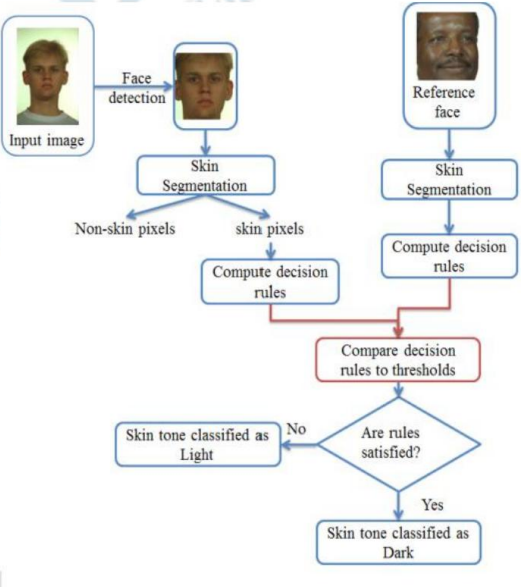
\includegraphics[]{Template_Latex_TCC-UNIFTEC/_lib/imagens/human_skin_detection.png}

\label{fig:x human_detection}
\centering{\Fonte{\cite{Human_Skin_Tone_Detection}.}}
\end{figure}

Para a etapa de reconhecimento facial, é necessário identificar a face na imagem carregada e segmentar a imagem para separar regiões com a presença e a não presença de pele. Para isto, foi substituído o modelo Gaussiano por não apresentar precisão mínima, apesar de sua simplicidade, e passou-se ao modelo elíptico. O modelo de limite elíptico utiliza a técnica de compensação de iluminação para corrigir o viés de cor e converter os componentes do modelo RGB para o espaço de cor YCbCr. Em seguida, os pixels de tom de pele são detectados por meio de um modelo de pele elíptico no novo espaço de cor. Os pixels detectados são segmentados iterativamente com base na variação de cor local, agrupados em pixels de coloração semelhante da região analisada, no caso, o rosto, considerando o arranjo espacial desses componentes e a semelhança de suas cores. Assim, o módulo de detecção de características faciais rejeita regiões candidatas de rosto que não contenham nenhuma característica facial, como olhos, boca e contorno facial. Após o processamento da imagem, as características são extraídas do conjunto de imagens e as cores são comparadas com as categorias propostas a partir de uma referência. Uma vez que a extração do tom de pele é realizada pelo algoritmo de aprendizado de máquina, os dados obtidos são enviados de volta ao servidor, são armazenados no banco de dados e, por fim, o resultado é exibido na página de \textit{front-end} para o usuário.

Como próximos passos, foi proposto primorar o sistema de reconhecimento de variação de cor facial adicionando pré-modelos mais detalhados e precisos e automatizar o processo para apresentar os resultados em um aplicativo web ou \textit{desktop}. Assim, como permitir o processamento em tempo real e adicionar o reconhecimento de outras variações de tons de pele, além dos tons comuns básicos. 

\section{Automatic Skin Tone Extraction for Visagism Applications}
 O estudo em \cite{Automatic_Skin_Tone_Extraction_for_Visagism_Applications}, propôs um sistema de classificação de pele em três tons, pele clara, média e escura para auxiliar na seleção de óculos, utilizando dois métodos.
 
O primeiro método utiliza as etapas convencionais do aprendizado de máquina com seleção da região de interesse, extração de características e classificação. Combinando e organizando vários espaços de cores em histogramas de manchas de pele e reduzindo o espaço de recursos resultante, de modo que apenas os recursos com alto poder discriminativo sejam mantidos para votação. Foi usado um classificador SVM treinado para rotular as cores de pele.

\begin{figure}[h]
\caption{Fluxograma de classificação por SVM }
\centering

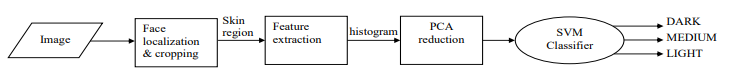
\includegraphics[]{Template_Latex_TCC-UNIFTEC/_lib/imagens/FluxogramaVisagismo.png}

\label{fig:x fluxogama_svm}
\centering{\Fonte{\cite{Automatic_Skin_Tone_Extraction_for_Visagism_Applications}.}}
\end{figure}

Primeira etapa do método é a identificação do rosto a partir da imagem e para isso foi utilizado o algoritmo Viola-Jones. Para evitar as partes irrelevantes como olhos, lábios e cabelos, foram cortadas as regiões de interesse (ROI) como abaixo dos olhos e acima do centro da face para melhor classificar o tom de pele. Em seguida, foi feito o vetor de características composto por 13 histogramas (3 espaços de cores e tons de cinza) baseado nos resultado dos quatro sistemas de cores, sendo eles RGB, HSV, Lab e YCrCb. A partir disso os dados alimentar o SVM para obter o tom de pele da região dominante no ROI.

O segundo método utiliza \textit{Deep Learning} com os estágios clássicos de aprendizado de máquina substituídos
pela rede neural convolucional (CNN) para extrair automaticamente recursos cromáticos de conjuntos aumentados de imagens faciais. Ambos os algoritmos foram treinados e testados em conjuntos de dados disponíveis publicamente. 

Para a CNN foi utilizada a rede VGG-19 que foi treinada previamente para reconhecimento de gênero a partir de imagens faciais com uma base de 200.000 imagens. Para detectar tom de pele, as duas ultimas camadas da CNN foram removidas para a parte restante ser usava como um extrator de recursos. Por fim, um classificador linear foi treinado para o problema de classificação de tom de pele utilizando as características previamente aprendidas pela CNN.

Para as etapas de treinamento e teste para ambos os métodos foram utilizadas imagens faciais da Internet e de diferentes bancos de dados disponíveis publicamente como Caltech, Chicago Face, Minear-Park e banco de dados de faces brasileiras por Thomaz e Giraldi. Cada banco possui diferentes características como controle ou não de ambiente e iluminação. Além de usar imagens faciais de celebridades selecionadas.

Para determinar o tom de pele real, cada amostra de imagem foi anotada independentemente por três pessoas
diferentes e o tom definido pela fusão dos resultados das anotações independentes. Primeiramente, os anotadores tiveram um treinamento com um especialista visagista que os instruiu com as regras que dois seguem no processo de anotação. Durante o treinamento, eles também anotaram com o visagista um subconjunto das imagens e discutiram como lidar com casos, limite e incertezas. Após mesclar os resultados de rotulagem humana, observaram que a maioria das
inconsistências de anotação apareceram entre os tons de pele médios e escuros.

Para melhorar a precisão foram utilizadas técnicas de aumento de contraste e aumento de brilho. O que tornou o algoritmo de aprendizado mais robusto para condições de iluminação. Com isso, o método SVM atingiu a precisão de 86,67\%, enquanto a abordagem CNN obteve uma precisão de 91,29\%. Contudo, foi possível apontar que no método CNN houve mais classificações errôneas entre cores médias claras e médias escuras, o parecido com a classificação conduzida por humanos anteriormente ao longo do estudo. Já na SVM não houve confusões entre cores escura e clara.

\section{Classification Algorithm for Skin Color (CASCo): Anew tool to measure skin color in social science research}
No artigo \cite{Classification_Algorithm_for_Skin_Color_CASCo_A_new_tool} os autores apresentam um algoritmo de classificação para cor de pele, chamado CASCo (\textit{Classification Algorithm for Skin Color}),  que permite identificar e classificar tons de forma objetiva, automática, acessível e personalizável, sem distorções de viés e preconceito racial. A metodologia proposta envolve revisar métodos tradicionais para a medição de tom de pele e observar suas deficiências e a partir disso construir uma ferramenta. Como resultado obteve-se o CASCo, uma biblioteca desenvolvida na linguagem Python que detecta o rosto, segmenta a pele e utiliza k-means para determinar a categoria de tom de pele de imagens.  

Para a detecção de tom de pele a biblioteca realiza a partir de fotos a detecção de face utilizando o sistema HSV para mapear as cores do rosto. O sistema HSV foi escolhido, pois ele é um sistema alinhado à percepção visual que os humanos possuem com relação às características das cores. 
O segundo passo extrai áreas que não contém pele utilizando \textit{threshold} do modelo HSV para restringir, no filtro da função de\textit{ blur} de Gaussian, apenas pele, retirando olhos, cabelos e dentes. Em seguida é utilizado o k-means para identificar duas cores como dominantes.
Como consequência, para categorizar as cores dominantes, é utilizada uma paleta como referência e calculada qual a cor detectada é mais próxima ao peso mínimo Delta E(CIE 2000), ou seja, qual a menor distância delta entre a paleta utilizada e o delta.
A paleta de referência padrão é a paleta PERLA. PERLA é uma paleta que contem 11 tons de pele como referência desenvolvida na Universidade de Princeton visando ajudar estudos de tons de pele na América Latina e já vem sendo utilizada na pesquisa social.Contudo, a biblioteca CASCo aspira ser configurável e a paleta a ser utilizada pode ser facilmente alterada.
Após a implementação, o CASCo tem como resultado a criação de um arquivo de relatório que contém nove colunas com as informações coletadas, sendo elas a imagem avaliada, a localização da face encontrada, a primeira cor dominante identificada e a segunda e as suas proporções de presença da cor da na área facial identificada, a cor PERLA identificada e a distância entre a cor dominante e a cor classificada calculada de 0 a 100. Além disso, é obtido através da modalidade de \textit{debug} a foto utilizada com o resultado da identificação facial e ao lado direito a paleta de cores dominantes e ao lado dela a paleta usada para a classificação com a cor classificada marcada. Abaixo é impresso o valor em hexadecimal da cor dominante e sua proporção e o hexadecimal da categoria da cor classificada e o valor resultante de acurácia. Como pode ser visto na Figura \ref{fig:x resultado_CASCo}.


\begin{figure}[h!]
\caption{Exemplo de resultados obtidos pelo processamento usando CASCo}
\centering

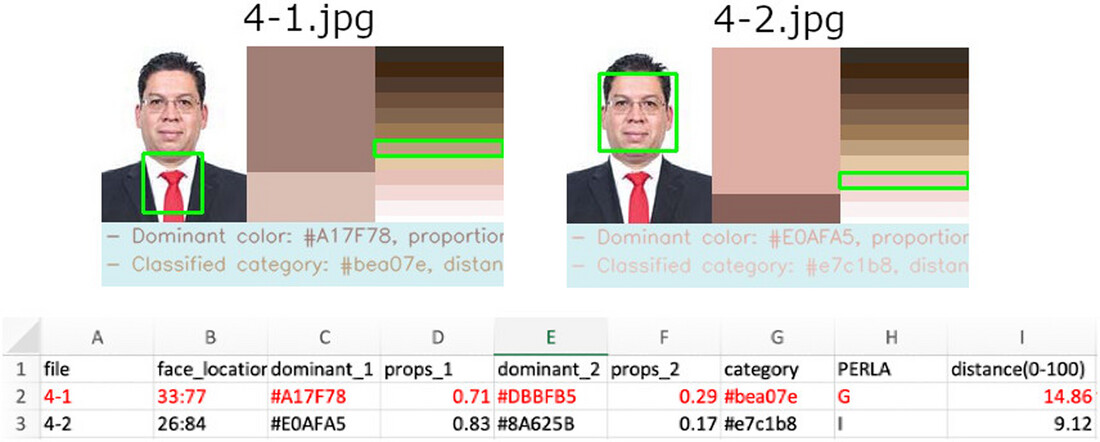
\includegraphics[scale=2]{Template_Latex_TCC-UNIFTEC/_lib/imagens/casco.jpg}

\label{fig:x resultado_CASCo}
\centering{\Fonte{\cite{Classification_Algorithm_for_Skin_Color_CASCo_A_new_tool}.}}
\end{figure}

Na modalidade de \textit{debug} as imagens processadas possuem seus resultados gerados anexados na pasta para verificação dos resultados, \textit{logs} gerados e a planilha \textit{result.csv} com o resumo de cada imagem.

Como fatores limitadores foram citados o próprio uso de imagens para a detecção, principalmente utilizando a pele facial que podem ter por natureza implicações relacionadas a problemas de capturamento e influência de iluminação nos tons de pele, apesar disso por ser uma alternativa barata comparada ao uso de espectrômetros isso seria facilmente burlado utilizando \textit{datasets} prontos reduzindo o esforço na coleta de imagens em novas pesquisas. Ademais, a CASCo possui limitações quanto a identificação caso a pessoa esteja usando maquiagem, por influenciar na correta amostra de pele e causar efeito de esbranquecimento nas peles.

Em suma, a CASCo é uma ferramenta que tem em vista democratizar a pesquisa relacionadas ao tom de pele, facilitando a viabilidade, replicabilidade e objetividade da medição de tons de pele. Apesar das limitações, por ser uma ferramenta customizável é possível introduzir novas paletas de classificação, novos clusters, quantidades de cores dominantes, etc. Também é uma ferramenta que pode processar rapidamente grandes \textit{datasets} de imagens e sem intervenção humana, além de não necessitar de aparelhos caros para medição como espectrômetros para seu funcionamento e ser disponibilizada para uso gratuitamente. Tudo é customizável, bastas os pesquisadores terem as cores hexadecimais ou as cores RGB para utilizar a biblioteca.



\section{Considerações sobre os trabalhos relacionados}

Recentemente, foi possível notar número limitado de trabalhos selecionados na área de identificação de tonalidade de pele, sobretudo pelo fato de a identificação de tom de pele não ser objeto final de muitos artigos, mas sim um dos processos para o reconhecimento facial bem-sucedido. 

Os artigos selecionados procuram identificar tonalidades de pele que não estão concentradas em regiões específicas ou em raças e etnias específicas. Contudo, a seleção se justifica porque a maioria utiliza a área facial para a identificação de tons de pele. Entre eles há escolha de faixas de cores de classificação diferentes, como a utilização do Guia Pantone de Tom de Pele, utilizado pela indústria, a paleta PERLA, criada com base no autorreconhecimento de raça e etnia na América Latina e a classificação classifica do visagismo como de pele clara, média e escura.

Apenas dois trabalhos utilizavam paletas de classificação em comum, contudo entende-se que entre os trabalhos relacionados dificilmente uma paleta irá abordar todos os tons de pele possíveis. Assim como, quanto mais cores forem colocadas para a classificação, mais erros de classificações entre tons parecidos podem ocorrer, como visto no primeiro artigo \cite{Facial_skin_colour_classification_using_machine_learning_and_hyperspectral_imaging_data}. Além disso, principalmente, ao usar humanos no estudo para validar classificações, pode desenrolar influência de viés históricos, étnicos e raciais. Ou seja, mesmo em uma paleta de três tons, uma pessoa em diferentes lugares pode ser classificada por pessoas em diferentes tonalidades, ao ser um tópico também subjetivo.

Com relação ao uso de sistema de cores, os mais usados foram os sistemas YCbCr e HSV, por serem modelos amplamente comuns na detecção de pele e que apresentam melhor resultado comparados aos outros modelos conhecidos. Quanto aos algoritmos de \textit{machine learning} e ferramentas, notou-se maior uso do algoritmo de Viola-Jones, principalmente por ser usadas fotos de rostos em três estudos, SVM e K-means. Além disso, dois dos trabalhos apresentaram valores de precisão superiores a 90\%.

A partir destas constatações, considerou-se que apesar de diferentes ferramentas, os desafios eram equivalentes, sendo possível resumir quais os pilares fundamentais para a implementação do trabalho. Sendo eles, coletar diferentes imagens de pele, tratar imagens considerando problema relacionados a iluminação, escolher sistemas de cores adequados para conversão das imagens e excluir e separar de regiões de pele e não pele nas imagens.


